% !TeX root = paper.tex
%%% TeXのファイル名を変えたら ↑ も変えましょう

% TEX STUDIO MAGIC-COMMAND
% !TeX document-id = {21ffa6e2-6c8f-4532-897c-386dc477f19a}
% !TeX root = paper.tex
% !TeX encoding = utf8
% !TeX TXS-program:compile = lualatex -file-line-error -synctex=1 -interaction=nonstopmode -halt-on-error %.tex
% !TeX TXS-program:quick = txs:///compile | txs:///view-pdf-internal --embedded
%%%-------------------------------------------------------------------------
%%% PD3レポートテンプレート
%%% 作成: 金沢工大・情報工学科・鷹合研究室
%%%-------------------------------------------------------------------------
\documentclass[a4paper,openright]{ltjsbook} 

\usepackage{takagolab}	% 鷹合研の設定
\newcommand{\red}[1]{\textcolor{red}{#1}}



\begin{document}
% !TeX root = paper.tex

\begin{titlepage}
 \begin{center}
  ~\\
  \vspace{1cm}
  {\Large 
  令和4年度\\
 プロジェクトデザインIII\\
  プロジェクトレポート\\
情報工学科\\}
  \vspace{1.3in}
  {\Huge \gtfamily
電車の分類をしたよ\\
  }
  \vspace{2in}
  {\LARGE 
  提出日~~~令和99年~99月~99日\\
  \vspace{0.4in}
  指導教員~:~鷹合 大輔 准教授\\
 \vspace{0.9in}
  氏名 学籍番号 (クラス--名列番号)\\
  \vspace{2mm}
  野崎 悠度 1936463 (4EP1--68)\\
  奥野 細道 1936119 (4EP4--75)\\
  }
 \end{center}
\end{titlepage}
 %タイトル
\frontmatter % タイトルの次に1ページの空きページを
% TEX STUDIO MAGIC-COMMAND
% !TeX document-id = {21ffa6e2-6c8f-4532-897c-386dc477f19a}
% !TeX root = abstract.tex
% !TeX encoding = utf8
% !TeX TXS-program:compile = lualatex -file-line-error -synctex=1 -interaction=nonstopmode -halt-on-error %.tex
% !TeX TXS-program:quick = txs:///compile | txs:///view-pdf-internal --embedded
%%% TeXのファイル名を変えたら ↑ も変えましょう



%%%-------------------------------------------------------------------------
%%% PD3予稿集テンプレート (main.tex)
%%% 作成: 金沢工大・情報工学科・鷹合研究室(2022,01/12)
%%%-------------------------------------------------------------------------

%%%%%%%%%%%%%%%%%%%%%%%%%%%%%%%%%%%%%%%%%%%%%%%%%%%%%%%%%%%%%%%%%%%%%%%%%%%
%                               テーマ,著者情報をここに書き込んでください
%ここから ------------------------------------------------------------------

%%% テーマ番号
\def\THEMEID{1EP001}

%%% タイトル
\def\TITLEJP{機械学習用いた電車の車両タイプの判別システムの開発}
\def\TITLEEN{Development of a train car type identification system using machine learning}
\def\CENTERADJ{3.3} % ここを書き換えて,表紙の「プロジェクトテーマ」という文字列がセル中心になるよう調整してください

%%% 教員名
\def\PROFNAME{鷹合 大輔 准教授}

%%% アブストラクト(英文で書く)
% 最低:100ワード,最大:300ワード前後
% 英文部分については,句読点は半角にすること.つまり", "か". "を使う
\def\ABSTRACT{
Describe about 5 lines of abstract in English here. Describe about 5 lines of abstract in English here. Describe about 5 lines of abstract in English here. Describe about 5 lines of abstract in English here. Describe about 5 lines of abstract in English here. Describe about 5 lines of abstract in English here. 
\textbf{(何が問題で,それをどんな手法で取り組んで,どういう結果であったかなどを英語で要約して下さい)}
 Describe about 5 lines of abstract in English here. Describe about 5 lines of abstract in English here. Describe about 5 lines of abstract in English here.
}

%%% キーワード(5個まで)
\def\KEYWORDS{YOLO,Machine Learning,Qwerty3,Qwerty4,Qwerty5}

%%% 著者リスト
\def\AUTHORS{
\begin{minipage}{13.5cm}
~\hfill 4EP1-68~野崎 悠渡(NOZAKI Yuto)      ~~~~~ 4EP5-11~田村 優祐(TAMURA Yusuke) \hfill~
\end{minipage}
}

\newcommand{\red}[1]{\textcolor{red}{#1}}


% テーマ,著者情報ここまで -----------------------------------------------------


%%%%%%%%%%%%%%%%%%%%%%%%%%%%%%%%%%%%%%%%%%%%%%%%%%%%%%%%%%%%%%%%%%%%%%%%%%%%
%                                本文


\documentclass{tkglabs}

\usepackage{caption}

\begin{document}
\maketitle
\begin{multicols*}{2} % *アスタ付きだとページのバランシングを無効にできる
%本文ここから ------------------------------------------------------------------



\section{はじめに}
%背景や目的をここに書いてください.
電車の車両タイプはJRの在来線だけでも100種類近く存在している.
多くの人は電車を見て電車だと認識することは可能だが,その電車の車両タイプまでを判断できる人は少ない.
電車についての知識がある人は一目見るだけでその電車の車両タイプを判断できるが,大多数の人は似ている電車の車両タイプを判断することが難しい.本プロジェクトでは簡単に画像や動画に写っている車両タイプが何なのかを判別できるシステムを開発する.

%\section{関連研究?現存するサービスについて?これいる??}
%先行事例と本システムの独自性
%googleがgoogleレンズというサービスを提供している.これは,画像に写っている物体と同じものが写っているウェブサイトをまとめて表示するサービスである.このサービスの問題点は3つある.
%\begin{itemize}
%	\item 一枚の画像に複数の物体が写り込んでいると判別結果が正確ではなくなる.
%	\item 提示されたウェブサイトから詳細を確認しなければならない.
%	\item 動画から物体を判別することができないこと
%\end{itemize}

\section{システム概要}
開発するシステムの概要を図 \ref{abc}に示す.
\begin{figure} % 小さな図
	\label{abc}
	\centering
	\includegraphics[width=\linewidth]{obj/system.pdf}
	\figcap{後で変える}{System Overview}{abc}
\end{figure}

\section{判別モデルの開発の流れ}
電車が写っている画像を集めて,データセットを作成し,学習をするという流れで判別モデルを開発する.

\subsection{データ収集}
	YouTubeで特定の電車のみが映っている1〜3種類の動画を保存して,指定した枚数のランダムなフレームを保存する.保存した画像を識別して,	電車が映っている画像だけを保存する.
	動画ごとに電車が写っている時間が異なるため,集めた画像は車両タイプごとに異なる.
	%各車両タイプが名前になっているディレクトリに保存する.
	各車両タイプの保存枚数を図\ref{fig:chart}に示す.
	
	% TODO: \usepackage{graphicx} required
	\begin{figure}
		\centering
		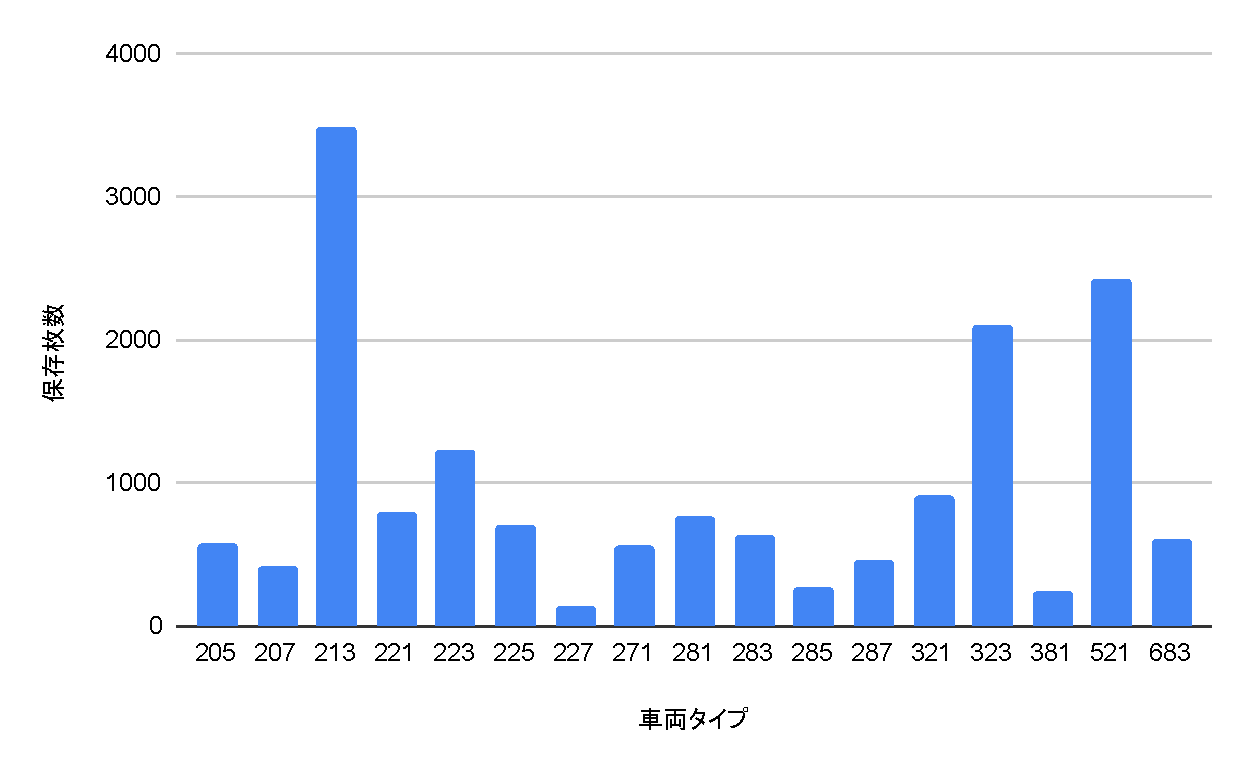
\includegraphics[width=\linewidth]{obj/chart.pdf}
		\figcap{各車両タイプの保存枚数}{Number of images saved by vehicle type}{fig:chart}
%		\label{fig:chart}
	\end{figure}
\subsection{データセットの作成}
本プロジェクトで作成するモデルは識別モデル,分類モデルの二種類である.%データセットのディレクトリ構造が識別用と分類用で異なるので,それぞれのデータセットを作成した.識別モデルには画像のアノテーション情報も必要なので,アノテーションを行い,識別モデル用のデータセットを作成した.
分類モデルのデータセット内の画像をアノテーションして識別モデル用のデータセットを作成した.
様々なウェブサイトから手作業で17種類の各車両の画像を10枚ずつ集めて,テストデータセットも作成した.


\subsubsection{分類とは}
%画像には何が写っているのかを判断することを分類という.一枚の画像に一つの物体が写っている場合に分類ができる.
分類はデータやオブジェクトを異なるクラスやカテゴリに分けるプロセスを指す.画像の分類とは,画像が特定のカテゴリやクラスに属するかどうかを判別する作業である.例えば,画像に写っているのが猫か犬か,車か飛行機かなどのクラスに分類することがある.
\subsubsection{識別とは}
識別とは画像のどこに何が写っているのかを判断するプロセスを指す.1枚の画像に複数の物体が写っていても識別はできる.

\subsubsection{アノテーションとは}
%https://www.dir.co.jp/world/entry/solution/annotation
アノテーションとは、機械学習の分類の一つである教師あり学習において,分析対象データにラベルを付与するプロセスである.画像にバウンディングボックスと呼ばれる四角形を描画しクラス番号を指定する.バウンディングボックスを描画することでその画像に写っている物体の座標情報を取得することができる.クラス番号とは,判別したいものリストを作成し,画像に写っている物体に対応した,リストのインデックスのことである.アノテーションをした結果は,識別モデルの学習時に使用する.
%\subsubsection{分類モデル}
%分類モデルのデータセットは,分類したいものの画像をそれぞれの車両タイプの名前のディレクトリに保存する.

%\subsubsection{識別モデル}
%識別モデルのデータセットは,学習用とテスト用の2種類のディレクトリのそれぞれに画像と画像のアノテーション情報が記載されているテキストファイルを保存する.画像ファイルとそのアノテーション情報のテキストファイルはファイル名を統一する必要がある.\\
%どんなふうにアノテーションをしたのか説明が必要?\\
%アノテーション情報には,クラス番号と画像で物体が写っている部分の座標情報が必要である.
%本プロジェクトにおける識別モデルのクラス番号は,リスト形式で識別したい車両タイプを定義した,それぞれの車両タイプのインデックスとした


\subsection{モデルの学習}
%本プロジェクトでは\\
YOLOv8を用いてモデルを作成した.
\subsubsection{YOLOv8の概要}
YOLOとはYou Only Look Onceの略で,人間のように一目見るだけで物体検出ができることを指している.データセットを作成し学習させることで,任意の物体のみ検出させることが可能である.
YOLOv8はYOLOシリーズの最新バージョンであり,ディープラーニングとコンピュータビジョンの最先端の進歩に基づいており,速度と精度の麺で比類のない性能を提供している.
%https://docs.ultralytics.com/ja/ 参照


\subsubsection{学習の実行}
学習を進めると徐々に性能が上がっていき性能が向上しなくなると学習が途中で中断される.
学習は中断されるまで続けたため,学習回数はモデルによって差がある.

\subsection{モデルの使い方}
識別モデルと分類モデルをどのように使えば結果が出力されるのかを説明する.pythonのコードを貼り付ける?
田村のパートに記載してもいいかもしれない
\section{作成したモデルの評価}
%\subsection{モデルの性能評価指標}
%本プロジェクトで作成する分類モデルは混合行列から性能の評価を行う.混合行列とは実際のデータと予測データを比較するためのもので,正しくラベル設定ができているのか,及び予測の精確度を把握することができる.

\subsection{分類モデルの性能評価}
作成した分類モデルを用いてテストデータセットの分類を行った結果を図\ref{fig:classifyresults}に示す.
\begin{figure}
	\centering
	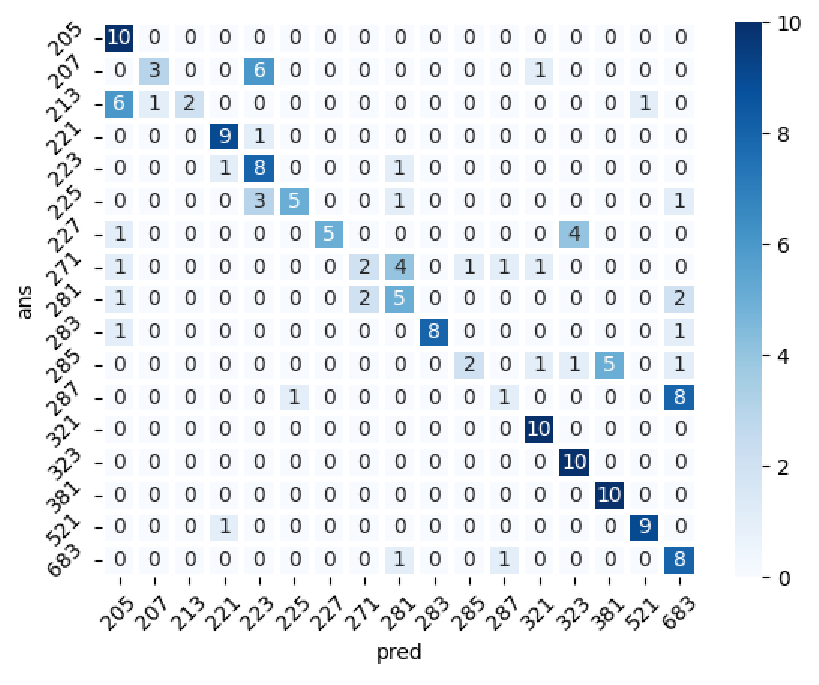
\includegraphics[width=\linewidth]{obj/classify_results.pdf}
	\figcap{性能評価}{seinouhyouka}{def}
	\label{fig:classifyresults}
\end{figure}

\subsection{識別モデルの性能評価}
%17種類の車両タイプの画像をそれぞれ10枚ずつ集めテストデータを作成し識別を行った.識別の結果を表\ref{detection}に示す.
%captionを追加するとエラーが発生してしまう
作成した識別モデルを用いてテストデータセットの識別を行った結果を図\ref{fig:chartdet}に示す.
識別失敗とは間違った車両タイプだと判断していることを指し,識別不能とはどの車両タイプにも当てはまらないと判断していることを指す.
% TODO: \usepackage{graphicx} required
\begin{figure}
	\centering
	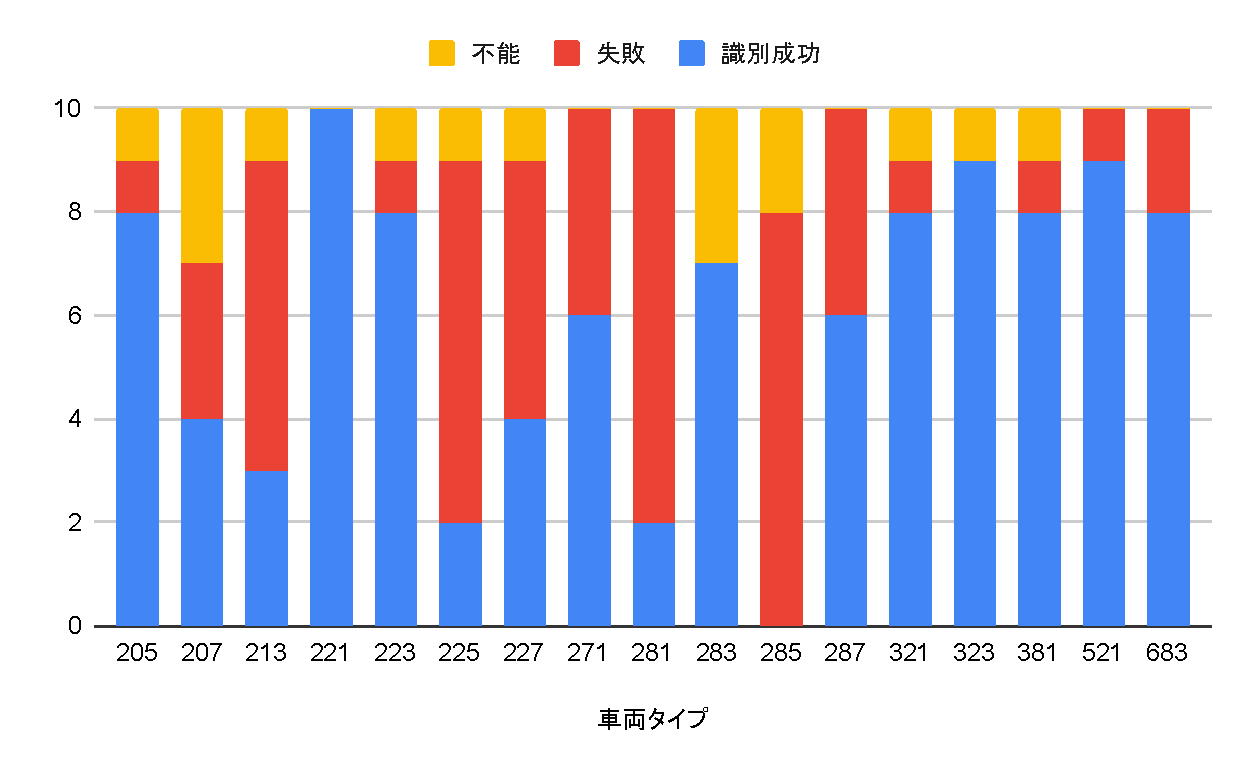
\includegraphics[width=\linewidth]{obj/chartDET.pdf}
	\figcap{テストデータ識別結果}{ababefn}{}
	\label{fig:chartdet}
\end{figure}





\section{考察}
正解率は電車によって異なることがわかる.特に外見が似ている電車だと,誤判別していることが多かった.%データセットの画質を落とすと誤判別が増えた.特に誤分類が多かった三種類の電車の画質を上げても結果はあまり変わらなかった.

%限られたストレージでは,データセットの画質を変化させて判別結果を向上させることは難しいと考えられる.SSDの容量に制限がない場合,大量の高画質のデータでデータセットを作成することで判別結果が改善される可能性があると考えられる.
各車両タイプの画像の枚数に差があったことが判別結果に影響を与えていると考えられる.
画像の枚数が少ない車両タイプの判別結果が必ず悪くはならなかった.
画像の枚数が判別結果に影響を与えるのではなく,車体の特徴が鮮明に写っている画像の枚数が判別結果に影響を与えると考えられる.データセットとして質の悪い画像を大量に集めるのではなく,車体の特徴が鮮明に写っている画像を車両タイプごとに集める必要があったと考えられる.\\


------------------ここまで野崎------------------\\
------------------ここから田村------------------\\
\section{システムについて} 

\subsection{システムの動作要件} 本システムでは,ノートパソコンにLinuxサーバのセットアップを行い,サーバとして使用した. ネットワークは,学内の固定IPを割り当ててもらい,学内ネットワークを使用した. 
サーバのスペックは以下の通りである.
\subsubsection{サーバのスペック} 
\begin{itemize} 
	\item OS: Ubuntu 22.04.3 LTS 
	\item メモリ: 4GB 
	\item CPU: Intel® Core(™) i7 
	\item GPU: NVIDIA GeForce GTX 470M \item HDD: 80GB 
\end{itemize}
\subsection{システムの開発環境} 本システムの開発には,以下の言語やツールを使用した.
\subsubsection{使用言語} 
\begin{itemize} 
	\item フロントエンド: 
	\begin{itemize} 
		\item html 
		\item JavaScript 
		\item css 
	\end{itemize} 
	\item バックエンド: 
	\begin{itemize} 
		\item JavaScript (Node.js) 
		\item Python 
	\end{itemize} 
\end{itemize}
\subsubsection{使用ツール} 
\begin{itemize} 
	\item エディタ: VSCode 
	\item ブラウザ: Google Chrome 119 
\end{itemize}

\subsection{システムの機能詳細} 本システムは,以下の3つの機能を提供する.
\subsubsection{電車の画像の分類} この機能では,ユーザがブラウザからアップロードした画像に含まれる電車の種類を分類する. 分類の結果,最も可能性が高いものをHTMLページに出力する.
\subsubsection{電車の画像の識別} この機能では,ユーザがブラウザからアップロードした画像に含まれる電車の位置と種類を識別する.  識別の結果,バウンディングボックスが追加された画像をHTMLページに表示する.
\subsubsection{電車の動画の識別} この機能では,ユーザがブラウザからアップロードした動画に含まれる電車の位置と種類を識別する. 識別の結果,バウンディングボックスが追加された動画をHTMLページに表示する.


\section{システムの速度検証}
画像・動画の解像度、各機能ごとの応答速度(解像度の調整が困難なためスマホのサイズでの検証にはしない)
(GPUで動作した際にはGPU固定)
GPUマシンが動作した場合、解像度一定で、各機能のCPU,GPU速度を検証
\subsection{システムの考察(GPU動作時)(仮)}
GPUを使用したときとCPUを使用したときでは動作の速度が大きく異なることが分かる。また、入力された画像や動画の解像度によっても速度が異なることが分かった。
\subsection{システムの考察(GPU非動作時)(仮)}
入力された画像や動画の解像度によっても速度が異なることが分かった。
\section{システムの考察}


------------------ここまで田村------------------\\

\section{まとめ}



%% 参考文献(必要に応じて追加)
\begin{thebibliography}{99}
%\bibitem{jp2k1} 織田 信長, 明智 光秀, "JPEG2000画像符号化システムにおける係数ビットモデリングと適応算術符号化,"Journal of signal processing(基礎シリーズ), vol.7, no.4, pp.257-266, July 2003.
%\bibitem{sdkguide}Parrot, "AR.Drone Developer Guide SDK 2.0"
%\bibitem{bk1} "金沢の暮らし", \url{http://www.kanazawa-it.ac.jp}
%\bibitem{bk2} 山田 太郎, "金沢の一人暮らし", トンチンカン出版, 2016.
\bibitem{bk0}"Ultralytics YOLOv8 ドキュメント",\url{https://docs.ultralytics.com/ja}
\bibitem{bk1}"アノテーションとは - 定義と重要性,必要な準備や注意点を解説",\url{https://www.dir.co.jp/world/entry/solution/annotation}
\end{thebibliography}

%\noindent\textbf{本プロジェクトに関する業績} % 学部
% \noindent\textbf{本研究に関する業績} % 院生の場合
%\begin{enumerate}[label=\arabic*),leftmargin=2.25\zw]
%\item 鈴木 大志 , 鷹合 大輔 , 中沢 実,"AutoVCを用いたゼロショットリアルタイム声質変換手法の提案",2021-DPS-189(5), 1-6 (2021-12-13) , 2188-8906.
%\end{enumerate}

% 本文ここまで ------------------------------------------------------------------
\end{multicols*} 
\end{document}

  % アブストラクト
% !TeX root = paper.tex


\thispagestyle{empty}

\begin{table}[tbp]
\large
\centering

% 活動履歴

	

{\gtfamily 活動履歴} 野崎 悠渡\\
\begin{tabular}{rlr}
\hline
\multicolumn{1}{c}{{\gtfamily 期間}}&
\multicolumn{1}{c}{{\gtfamily 活動内容}}&
\multicolumn{1}{c}{{\gtfamily 活動時間[h]}}
\\
4--8月 & 調査・実験・実装 & 200 \\
11--3月 & 実験・実装・論文執筆(\ref{genri}章) & 160\\
\hline
\end{tabular}\\
\vspace{2in}
{\gtfamily 活動履歴} 鬼 太郎\\
\begin{tabular}{rlr}
\hline
\multicolumn{1}{c}{{\gtfamily 期間}}&
\multicolumn{1}{c}{{\gtfamily 活動内容}}&
\multicolumn{1}{c}{{\gtfamily 活動時間[h]}}
\\
4--8月 & 調査・実験・実装 & 200 \\
11--3月 & 実験・実装・論文執筆(\ref{genri}章) & 160\\
\hline
\end{tabular}\\

\end{table}
\clearpage
 % 活動履歴と作業分担

\mainmatter %ここから本文(<--これないと目次のページがずれる?)
% !TeX root = paper.tex

\pagenumbering{roman}		% ページ番号をローマ数字に
\setcounter{tocdepth}{3}
\tableofcontents			% 目次
\listoffigures				% 図目次
\listoftables				% 表目次
\lstlistoflistings	% ソースリスト目次
\clearpage
\pagenumbering{arabic}		% ページ番号をアラビア数字に
   % 目次,図目次,表目次,ソースリスト目次

% ★★★★★★★★★★★★★★★★★★★★★★★★★★★★★
\setcounter{page}{0} % PDFにしたときに,第1章が右ページからが始まらないときは,0にすること
% PDF印刷時の注意: ①実際のページ,②両面,③空白ページを除外しない, にすること.さもないと見開き時におかしくなる
% ★★★★★★★★★★★★★★★★★★★★★★★★★★★★★

% !TeX root = paper.tex


\chapter{序論}

電車の車両タイプは JR の在来線だけでも 100 種類近く存在している.
多くの人は電車を見て電車だと認識することは可能だが,その電車の車両タイプまでを判断できる人は少ない.
電車についての知識がある人は一目見るだけでその電車の車両タイプを判断できるが,大多数の人は似ている電車の車両タイプを判断することが難しい.
現在,車両タイプを調べる方法としてGoogle レンズを使用することや,図鑑と見比べる方法が挙げられる.
googleレンズは一枚の画像に2つ以上の電車が写っていると車両タイプを正確に分類できず,分類結果は車両タイプが出力されるのではなく,入力画像に写っているモノと似ているものが写っているウェブページ一覧を出力するので,出力されたウェブサイトを開いて知りたい情報を自分で探し出す必要がある.
図鑑と見比べる方法では知りたい情報を得るために多くの時間が必要になる.

現在の方法では画像に写っている車両タイプが何なのかが知りたいときに余計な手間をかける必要があるという問題がある.
本プロジェクトではこの問題を解決するために画像や動画に写っている車両が何なのかを判別できるシステムを開発する.

%序論には研究の背景と目的を書く.どういう問題があって,現在はどういう手法がとられているなど,先行研究で試みられている手法などを参考文献を交えながら書く.序論の終わりには,各章に何を述べたかを簡潔に記述する.
%現在,似ている電車がいっぱいある
%それぞれがどの車両タイプの電車なのかを判断したいよ
%画像を読み込ませることで,その画像には何が写っているのか判断するシステムを開発する\\
%画像に写っている電車が何なのかを判断するためには電車の図鑑と画像を見比べて,自分で判断する方法しかない.
%その車両が何なのか知るために大きな労力が必要であることが問題である.\\
%現在の画像分類では,画像に写っているのが,人や車,犬など,大まかな分類しかすることができない.
%この方法では電車の車両タイプが何かを判断することができない.\\
%本プロジェクトでは,電車が写った画像を与えることで車両タイプを判別するシステムを開発する.


 % 1章
% !TeX root = paper.tex


\chapter{システム概要}
\section{この章で書くこと}
\begin{itemize}
	\item 識別,分類とは
	\item 現存するサービスでできること
	\item 概要図
	\item モデルについて
	\item サーバ関連について
	%\item もしかしたらあんまり書くことないかも
\end{itemize}
\section{分類・識別とは}
\red{文の量が少ない?加えたほうが良いのか}\\
%参考文献:https://business.ntt-east.co.jp/content/cloudsolution/column-391.html
分類とは,画像に写っているものが何かを判断することである.\\
(例)犬,猫,電車,人\\
識別とは,画像に写っているものが何か,どこに写っているのかを判断することである.\\
(例)家族の集合写真で,自分がどこにいるのかを特定する.
\section{現存するサービス}
\red{箇条書きはやめたほうが良い?\\現在車両タイプを調べるためには,〜〜〜〜〜 のほうが良いのか}
\begin{itemize}
	\item Google レンズ
	\item YOLO
\end{itemize}

\subsection{Googleレンズ}\label{google-service}
これは画像の分類を行うアプリである.単に分類結果が表示されるのではなく,分類したいオブジェクトが映っているウェブサイト一覧が表示されるものである.表示されたウェブサイトを適当に選び自分が知りたい結果をウェブサイトの中から探し出す必要がある.また,一枚の画像に複数のオブジェクトが存在している場合は正しい結果が得られない.

%\subsection{YOLO}\label{YOLO-service}
%YOLOの説明いいいいい

%YOLOでは,学習データを準備し学習させることで任意のオブジェクトを判別できるモデルの開発ができる.
%本プロジェクトでは,YOLOを用いて電車の車両タイプを識別,分類する2つのモデルを開発する.




\subsection{YOLO}
YOLOとはYou Only Look Onceの略で,人間のように一目見るだけで物体検出ができることを指している.データセットを作成し学習させることで,任意の物体のみ検出させることが可能である.
YOLOv8はYOLOシリーズの最新バージョンであり,ディープラーニングとコンピュータビジョンの最先端の進歩に基づいており,速度と精度の麺で比類のない性能を提供している.
%https://docs.ultralytics.com/ja/ 参照
本プロジェクトでは,YOLOv8を用いて電車の車両タイプを識別,分類する2つのモデルを開発する.

\section{システム概要図}
本プロジェクトで開発するシステム概要を図\ref{FIG}に示す.システムは車両判別部とUIに分けられる.\\
\red{田村と相談,画像は後で変える\\画像の場所は変えられないのか}

\begin{figure}
	\centering
	\includegraphics [width=\linewidth]{fig/system.pdf}
	\caption{システム概要図}
	\label{FIG}
\end{figure}






 % 2章
% !TeX root = paper.tex


\chapter{学習データの準備}\label{genri}
\section{この章で書くこと}
\begin{itemize}
	\item djangoの件
	\item 電車が映っている場面だけ画像で保存
	\item データセットを作成(識別・分類)
	\item アノテーションについて
\end{itemize}

\section{画像の収集}
学習データは,ある電車が映っているYouTubeの動画をダウンロードして,任意の枚数だけランダムでフレームを保存する.その後,保存した画像を識別して電車が映っている場面のみ画像で保存をした.
本プロジェクトでは,JR西日本の在来線の電車を識別または分類する.\\
205  207  213  221  223  225  227  271  281  283  285  287  321  323  381  521  683 \\
上記の17種類の画像を集める
\subsection{動画の保存方法}
動画の保存にはyt-dlpというものを使う.
1〜3種類の動画の任意の秒数をダウンロードしてそれぞれの動画を連結して一つの動画にするwebアプリをpythonのフレームワークの一つであるdjangoを使って作成した.\\
	\red{画像は後で変える,大きさを揃える}\\
	作成したwebアプリは,図\ref{test1} 図\ref{test2}  図\ref{test3}のようになっている.
	YouTube上の動画のURLと開始時刻(秒),終了時刻(秒),車両タイプ名を入力して,1〜3種類の動画を保存し連結して一つの動画にしている.
	
\begin{figure}
	\centering
	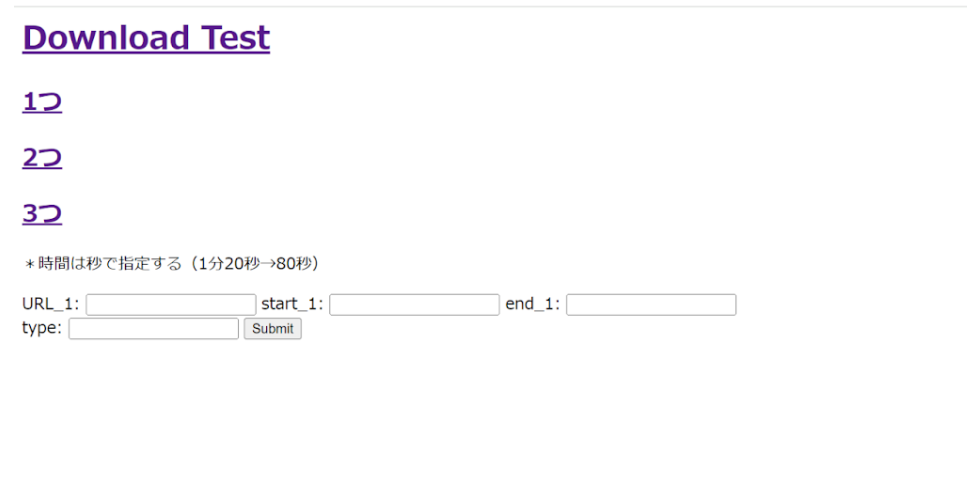
\includegraphics [width=\linewidth]{chap3/fig/test1.png}
	\caption{動画のダウンロード1}
	\label{test1}

	
	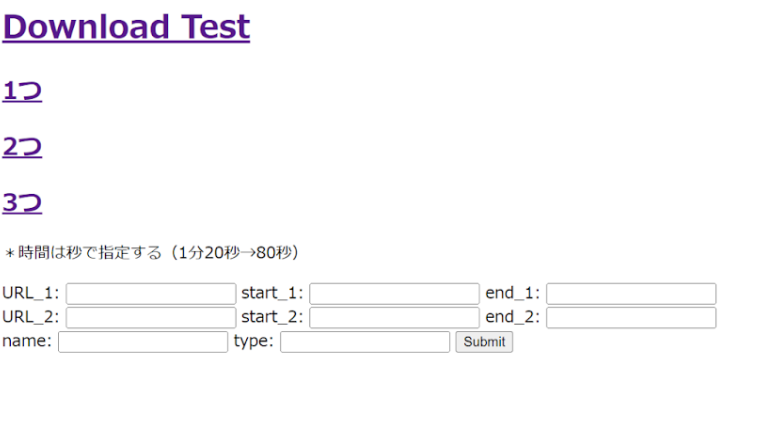
\includegraphics [width=\linewidth]{chap3/fig/test2.png}
	\caption{動画のダウンロード2}
	\label{test2}
	
	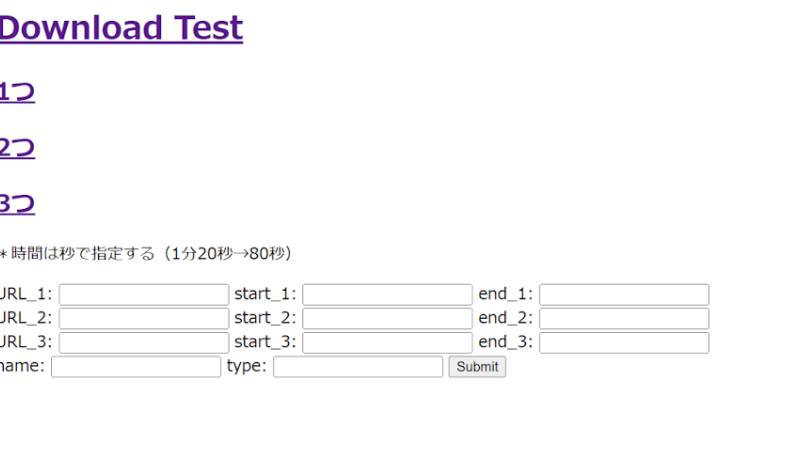
\includegraphics [width=\linewidth]{chap3/fig/test3.png}
	\caption{動画のダウンロード3}
	\label{test3}
\end{figure}

\subsection{画像の保存方法}
画像の保存は二回行う
一回目は,保存した動画でランダムなフレームを保存する.
二回目は,保存した画像を配布されているモデル(yolov8n.pt)で識別をして,電車が一つだけ映っているものだけを保存する.\\
\red{↓は消しても良いのか}\\
電車の画像を保存する際には,車両タイプ(数字3桁)というディレクトリに\\
車両タイプ(数字3桁)_通し番号(数字4桁).jpg    という名前で保存する
\section{データセットの作成}
\subsection{データセットの構造}
識別モデルと分類モデルでは学習時に使用するデータセットの構造がことなる.また識別モデル用のデータセットには画像のアノテーション情報が必要となる.
\subsection{アノテーション}
%https://www.dir.co.jp/world/entry/solution/annotation
アノテーションとは、機械学習の分類の一つである教師あり学習において,分析対象データにラベルを付与するプロセスである.画像にバウンディングボックスと呼ばれる四角形を描画しクラス番号を指定する.バウンディングボックスを描画することでその画像に写っている物体の座標情報を取得することができる.クラス番号とは,判別したいものリストを作成し,画像に写っている物体に対応した,リストのインデックスのことである.アノテーションをした結果は,識別モデルの学習時に使用する.\\
一般的にアノテーションは,手作業で行うものである.
しかし,数千枚の画像を手作業で行うことは難しいので,自動で行えるようにした.
分類モデル用のデータセットでは一枚の画像に電車が一つだけ映っている.その画像を配布されている識別用モデルで識別することでクラス番号と電車が映っている座標情報をテキストに書き込む.その後,本プロジェクトで識別する車両タイプリストに対応するクラス番号を上書きすることで,分類モデル用のデータセットから識別モデル用のデータセットを作成した.

\red{この章は他に書くことがあるのか}

 % 3章
% !TeX root = paper.tex


\chapter{車両タイプ判別モデルについて}
\section{この章で書くこと}
\begin{itemize}
	\item yoloとは
	\item 学習の実行
	\item 性能評価
	\item 作成したモデルの使い方
	\item 出力されるものについて
\end{itemize}

\section{YOLOとは}
YOLOの説明 \\
YOLOとはYou Only Look Onceの略で,人間のように一目見るだけで物体検出ができることを指している.データセットを作成し学習させることで,任意の物体のみ検出させることが可能である.\\
YOLOv8の説明   \\
YOLOv8はYOLOシリーズの最新バージョンであり,ディープラーニングとコンピュータビジョンの最先端の進歩に基づいており,速度と精度の麺で比類のない性能を提供している.
%https://docs.ultralytics.com/ja/ 参照

\section{学習の実行}
学習時にモデルの性能がそれまで以上に向上しなくなると学習が強制終了するため,エポック数という学習用データを何回繰り返して学習させるのかを表す数を10万回程度に設定して学習を進めた.強制終了した際のモデルが使用したデータセットで作れる最高の性能のモデルとなる.
\section{性能の評価}
\subsection{分類モデルの評価方法}
17種類の各車両の画像をそれぞれ10枚ずつ集めて画像の分類を行った.
分類モデルの予測した車両タイプと正解の車両タイプがどの程度あっているのか確かめることで性能の評価を行った.
\subsection{分類モデルの評価}
%分類モデルの評価を図\ref{CLS}に示す
\begin{figure}	
	\centering
	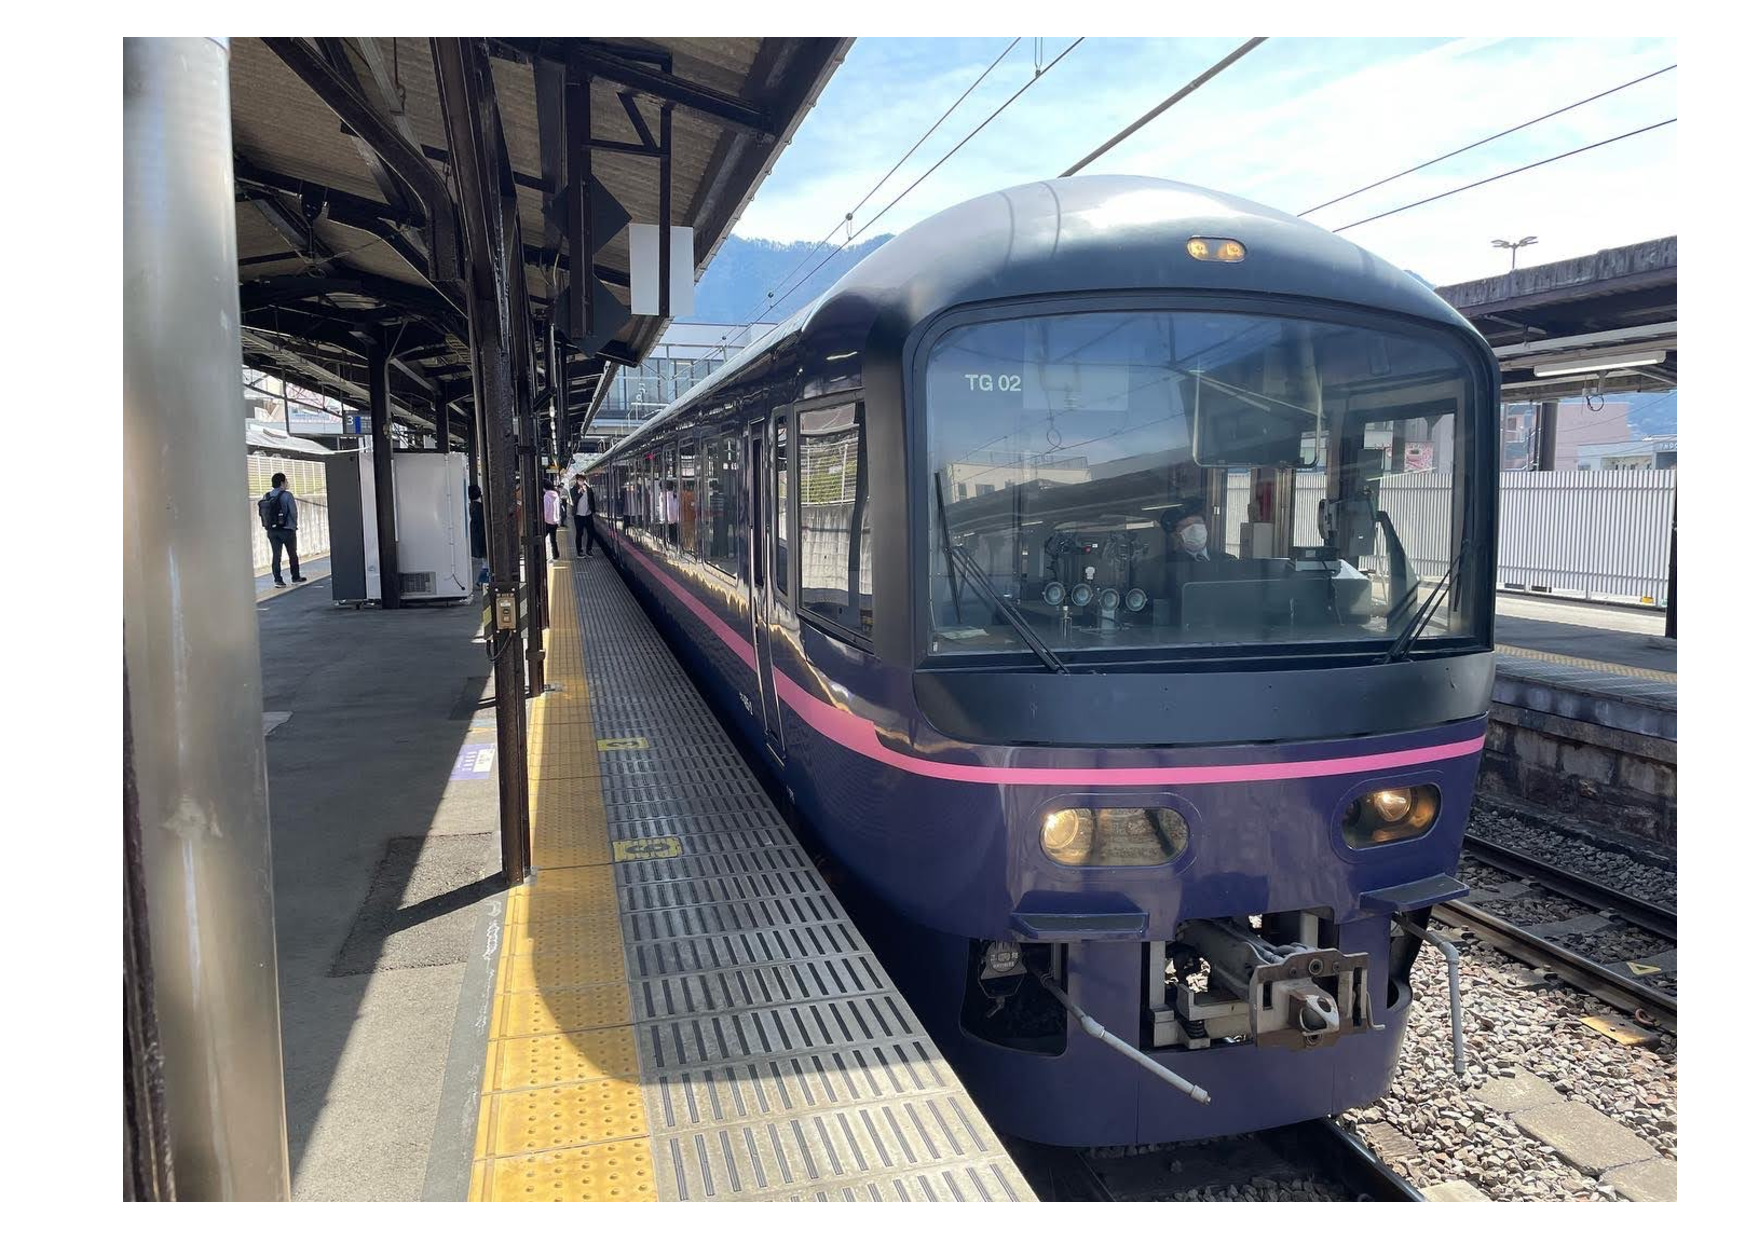
\includegraphics[width=\linewidth]{fig/hana.pdf}
	\caption{分類モデルの評価}\label{CLS}
\end{figure}
分類モデルの評価を図\ref{CLS}に示す.
縦軸が予測した車両タイプ,横軸が正解の車両タイプとするグラフである.
\subsection{識別モデルの評価方法}
作成した識別モデルは,次の指標から評価をする.\\
%https://qiita.com/panchoooon/items/2c972ede2bc883597a87

\begin{itemize}
	\item mAP(mean Average Precision)
	\item IoU(Intersection over Union)
\end{itemize}
\subsubsection{mAP}
%mAPの説明

\subsubsection{IoU}
IoUの説明

\section{作成したモデルの使い方}
識別モデルと分類モデルで使い方はほとんど同じ
作成したモデルをロードして,モデルに画像または動画を渡すと識別または分類をすることができる\\
識別
\begin{verbatimx}
$from ultralytics import YOLO
 model = YOLO("作成した識別モデルのパス")
 results = model.predict("画像のパス", save = True)
$
\end{verbatimx}

分類
\begin{verbatimx}
$from ultralytics import YOLO
 model = YOLO("作成した分類モデルのパス")
 results = model("画像のパス", save = True)
$
\end{verbatimx}
\section{出力されるもの} % 4章
% !TeX root = paper.tex


\chapter{結論}
あわれといふも,なかなか疎かなり.されば,人間の儚き事は,老少不定のさかいなれば,誰の人も早く後生の一大事を心にかけて,阿弥陀仏を深く頼み参らせて,念仏申すべきものなり. あなかしこ,あなかしこ.あわれといふも,なかなか疎かなり.されば,人間の儚き事は,老少不定のさかいなれば,誰の人も早く後生の一大事を心にかけて,阿弥陀仏を深く頼み参らせて,念仏申すべきものなり. あなかしこ,あなかしこ.あわれといふも,なかなか疎かなり.されば,人間の儚き事は,老少不定のさかいなれば,誰の人も早く後生の一大事を心にかけて,阿弥陀仏を深く頼み参らせて,念仏申すべきものなり. あなかしこ,あなかしこ.あわれといふも,なかなか疎かなり.されば,人間の儚き事は,老少不定のさかいなれば,誰の人も早く後生の一大事を心にかけて,阿弥陀仏を深く頼み参らせて,念仏申すべきものなり. あなかしこ,あなかしこ.あわれといふも,なかなか疎かなり.されば,人間の儚き事は,老少不定のさかいなれば,誰の人も早く後生の一大事を心にかけて,阿弥陀仏を深く頼み参らせて,念仏申すべきものなり. あなかしこ,あなかしこ.あわれといふも,なかなか疎かなり.されば,人間の儚き事は,老少不定のさかいなれば,誰の人も早く後生の一大事を心にかけて,阿弥陀仏を深く頼み参らせて,念仏申すべきものなり. あなかしこ,あなかしこ.
 % 5章

% !TeX root = paper.tex


\renewcommand{\bibname}{参考文献}
%\addcontentsline{toc}{chapter}{\protect\numberline{参考文献}}
%\addcontentsline{toc}{chapter}{参考文献}
\begin{thebibliography}{99}
\bibitem{1}V.D. Vaughen and T.S. Wilkinson, ''System considerations for
	multispectral image compression designs,'' IEEE Signal
	Process. Mag., vol.12, no.1, pp. 19-31, Jan. 1995.
\bibitem{2}A. Said and W. Pearlman, ''An image multiresolution representation
	for lossless and lossy compression,'' IEEE Trans. Image
	Process., vol.5, no.9, pp.1303-1310, Sept. 1996.
\bibitem{3}小野文孝, ''静止画符号化の新国際標準方式(JPEG2000)の概要,''映
	像情報メディア学会誌, vol.54, no.2, pp.164-171, Feb. 2000.
\bibitem{4}D. Tretter and C.A. Bouman, ''Optimum transform for multispectral
	and multilayer image coding,'' IEEE Trans. Image Process., vol.4, no.3, pp.296-308,
	March 1995.
\bibitem{5}F. Amato, C. Galdi and G. Poggi, ''Embeded zerotree wavelet
	coding on multispectral images,'' IEEE Proc. ICIP 97, vol.1, pp.612-615, 1997.
\bibitem{6}B.R. Epstein, R. Hingorani, J.M. Shapiro and
	M. Czigler, ''Multispectral KLT-wavelet data compression for
	Landsat thematic mapper images,'' Proc. Data Compression
	Conf., IEEE Computer Society Press, pp.200-205, 1992.
\bibitem{7}J.M. Shapiro, S.A. Martucci, and M. Czigler, ''Comparison of
	multispectral Landsat imagery using the embeded zerotree
	wavelet(EZW) algorithm,'' DLPO at Image Compress. Appli. \&
	Innovation Workshop, pp.105-113, March 1994. 
\bibitem{8}J.A. Saghri, A.G. Tescher, and J.T. Reagan, ``Practical transform
	coding of multspectral imagery,'' IEEE Signal Process. Mag.,
	vol.12, no.1, pp.32-43, Jan. 1995.
\bibitem{9}J. Lee, ``Optimized quadtree for Karhunen-Loeve transform in
	multispectral image coding,'' IEEE Trans. Image Process., vol.8, no.4,
	pp.453-461, April 1999.
\bibitem{10}B. Brower, B. Gandhi, D. Couwenhouven and C. Smith, ``ADPCM
	for advanced LANDSAT downlink applications,'' in Proc. 27th
	Asilomar Conf. Signals, Systems and Computers, Nov. 1993. 
\bibitem{11}N.D. Memom, K. Sayood and S.S. Magliveras. ,''Lossless compression
	of multispectral image data,'' IEEE Trans. Geosci. and
	Remote Sensing., vol.32, no.2 , pp.282-289, March 1994.
\bibitem{12}S. Gupta and A. Gersho, ``Feature predictive vector quantization
	of multispectral images,'' IEEE Trans. Geosci. and
	Remote Sensing., vol.30, no.3, pp.491-501, May 1992.
\bibitem{13}K. Irie and R. Kishimoto, ``A study on perfect reconstructive
	subband coding,'' IEEE Trans. Circuits Syst. Video Technol.,
	vol.1, no.1 , pp.42-48, March 1991.
\bibitem{14} 小松 邦紀, 瀬崎 薫, 安田 靖彦, ``濃淡画像の可逆的なサブ
	バンド符号化法'', 信学論(D-II), vol.J78-D-II, no.3,
	pp.429-436, March 1995.
\bibitem{15}A.R. Calderbank, I. Daubechies, W. Sweldens and B. Yeo, ''Lossless
	image compression using integer to integer wavelet transforms,'' 
	IEEE Proc. ICIP 97, vol.1, pp.596-599, 1997.

\bibitem{16}F.A.M.L. Bruekers and A.W.M.V.D. Enden, ``New networks for
	perfect inversion and perfect reconstruction,'' IEEE
	J. Sel. Areas Commun., vol.10, no.1, pp.130-137,
	Jan. 1992. 
%ブリューカとエンデン「ラダー回路による可逆変換」

\bibitem{17}小松 邦紀, 瀬崎 薫, ``可逆的離散コサイン変換とその画像情報圧
	縮への応用,'' 信学技報, vol.IE97-83, pp.1-6, Nov. 1997.
\bibitem{18}K. Komatsu and K. Sezaki, ''Design for lossless block
	transforms and filter banks for image coding,'' IEICE
	Trans. Fundamentals, vol.E82-A, no.8, pp.1656-1664,
	Aug. 2000.
\bibitem{19}福間 慎治, 岩橋 雅宏, 神林 紀嘉, ``可逆的色変換を用いた色彩
	画像の可逆符号化,'' 信学論(D-II), vol.J81-D-II, no.11, pp.2680-2684, Nov. 1998.
\bibitem{20} T. Nakachi, T. Fujii, and J. Suzuki,''A unified coding
	algorithm of lossless and near-lossless color image
	compression,'' IEICE Trans. Fundamentals, vol.E83-A, no.2,
	pp. 301-310, Feb. 2000.
\bibitem{21}仲地 孝之, 藤井 竜也, ``可逆KL変換を用いた病理顕微鏡画像符号
	化法の研究,'' 2000信学総大, D16-13, March 2000.
\bibitem{22}鷹合 大輔, 武部 幹, ``可逆WT・KLTを用いるマルチスペクトル画
	像の情報圧縮,'' 信学論(A), vol.J84-A, no.3, pp.1-11, March
	2001.
\bibitem{23}尾上 守夫, ``画像処理ハンドブック,'' 昭晃堂, pp.554-561, 1987.
\bibitem{24}鷹合 大輔, 武部 幹, ``マルチスペクトル画像のバンド間・バンド
	内相関除去による可逆情報圧縮,'' 第15回DSPシンポジウム講演論文集, pp.475-48, Nov.
	2000.
\bibitem{25}鷹合 大輔, 武部 幹, ``ウェーブレット変換を用いたマルチスペク
	トル画像の情報圧縮符号化法の研究,'' 平成10年度金沢工大卒業論文,
	1998.
\bibitem{26}酒井 幸市,``デジタル画像処理入門,'' コロナ社,1997.
\bibitem{27}榊原 進,``ウェーブレットビギナーズガイド,'' 電機大出版局,
	 1995.
\bibitem{28}武部 幹,``情報圧縮、通信と回路理論,'' 信学技報,IT97-40,July
	1997.
\bibitem{29}Gilbert Strang and Troung Nguyen,``
Wavelet and filter banks,' 'Wellesly Cambridge Press,1996.
\bibitem{30}貴家 仁志,``よくわかるディジタル画像処理,'' CQ出版社,1996.
\bibitem{bk1} "金沢の暮らし", \url{http://www.kanazawa-it.ac.jp}
\bibitem{bk2} 山田 太郎, "金沢の一人暮らし", トンチンカン出版, 2016.
 \end{thebibliography}
 
 % 参考文献
\newpage
% !TeX root = paper.tex


\appendix %付録
\chapter{開発したプログラム}
\section{セットアップ方法}


にプログラムの使い方,セットアップ方法などを書きましょう.ここにプログラここにプログラムの使い方,セットアップ方法などを書きましょう.ムの使い方,セットアップ方法などを書きましょう.
ここにプログラムの使い方,セットアップ方法などを書きましょう.

\begin{Verbatim}[frame=single]
$ sudo apt-get install python3-pip      # PIPコマンドの導入
$ echo "Hello WOrld"
Hello WOrld
\end{Verbatim}

にプログラムの使い方,セットアップ方法などを書きましょう.ここにプログラここにプログラムの使い方,セットアップ方法などを書きましょう.ムの使い方,セットアップ方法などを書きましょう.
ここにプログラムの使い方,セットアップ方法などを書きましょう.

\section{使い方}
ここにプログラムの使い方,セットアップ方法などを書きましょう.
ここにプログラムの使い方,セットアップ方法などを書きましょう.ここにプログラここにプログラムの使い方,セットアップ方法などを書きましょう.ムの使い方,セットアップ方法などを書きましょう.
ここにプログラムの使い方,セットアップ方法などを書きましょう.ここにプログラムの使い方,セットアップ方法などを書きましょう.
%%%%%%%%%%%%% プログラムの埋め込み %%%%%%%%%%%%%%%%%%%%%%%%%

\section{ソースコード}
%% ファイル名を指定して、挿入する場合
%\lstinputlisting[language=c,caption=サンプルプログラム,label=sample.c]{appendix/src/sample.c}
%project_processing.pyとsave.py
\lstinputlisting[language=Python,caption=画像の保存1,label=project_processing.py]{appendix/src/project_processing.py}
\lstinputlisting[language=Python,caption=画像の保存2,label=save.py]{appendix/src/save.py}


\chapter{いいいいい}
あああああああああああああああああああああいいいいいいいいいいいいいいいいいいいいいいいいいいいいううううううううううううううううう
     % 付録  listingsがうまくイカない

\end{document}
